\chapter{Spectral Method}
\label{chap:spectral-method}

% \section{Content}
% \input{chapters/out/Spectral Method.md.tex}

In this chapter we will construct a spectral method in the basis of Jacobi polynomials to explore the solution of equilibrium distributions $\rho(\vec{x})$.
Starting from a many-body system and considering the continuous limit as $N_p \goesto \infty$, in \Cref{chap:particle-interaction-theory} we have already established the governing equation of the particle density distribution $\rho(\vec{x})$ in such a system.

Can we put together a numerical method to solve for the equilibrium distribution (cf. \Cref{def:equilibrium-measure})?
Let us consider the problem from the bottom up and start from the solution:
The basic idea behind spectral methods is to assume a solution $\rho(\vec{x})$ of the form
$$\rho(\vec{x}) = \sum_{k=0}^{N-1} \rho_k \varphi_k(\vec{x})\,,\quad \rho_k \in \R, \varphi_k: \R^d \mapsto \R\,,\quad k = 0, ..., N-1\,,$$
with $N$ coefficients $\vec{\rho} := \left(\rho_0, ..., \rho_{N-1}\right)^T$ multiplying $N$ basis functions $\varphi_k$.

\section{Orthogonal Polynomials forming a Basis}
The following section will introduce a few necessary objects and tools to understand the basis of functions we are working with to construct the spectral method, the basis of Jacobi polynomials.

We start with the Pochhammer symbol, another name for the \textit{rising factorial}, an unusual notation for a function but standard in the context of the special functions that will be introduced on top of it.
\begin{definition}{Rising Factorial (Pochhammer Symbol)}{rising-factorial}
  The $n$th rising factorial of $x \in \R$ is given by
  $$(x)_n := \prod_{k=0}^{n-1} (x+k) \,\in \R\,.$$
\end{definition}

For example, $(3.141)_5 = 3.141 \cdot 4.141 \cdot 5.141 \cdot 6.141 \cdot 7.141$.

\begin{remark}{Nonpositive integer rising factorial}{nonpositive-pochhammer}
  When the argument is a nonpositive integer, the rising factorial
  $(-m)_n = -m \cdot (-m+1) \cdot ... \cdot (-m+n-1)$
  vanishes when $n \ge m+1$ for $n \in \N$ and $m \in \N_0$ as $0$ is among the factors.
\end{remark}


As a second prerequisite, we introduce closely intertwined beta- and gamma-functions.
\begin{definition}{Gamma Function}{gamma-function}
  Aligning with the factorial for integer arguments, $\Gamma: \R^+ \mapsto \R$ is given by
  $$\Gamma(x) := \int_0^\infty t^{x-1}\e^{-t} \ddt\,.$$
\end{definition}

\begin{definition}{Beta Function}{beta-function}
  $B: \R^+\times\R^+ \to \R$ is given by
  $$B(x_1, x_2) := \int_0^1 t^{x_1-1}(1-t)^{x_2-1} \ddt\,.$$
\end{definition}

Note that following from this definition, there is a relationship with the gamma-function
\begin{equation}
  B(x_1, x_2) = \frac{\Gamma(x_1) \Gamma(x_2)}{\Gamma(x_1 + x_2)}\,.
  \label{eq:beta-gamma}
\end{equation}


In order to efficiently construct a spectral method, we need an orthogonal basis.
\begin{definition}{Orthogonal Polynomials}{orthogonal-polynomials}
  Are univariate polynomials
  $$p_n: \R \mapsto \R, \; p_n(x) = \sum_{k=0}^{n} c_k x^k\,.$$
  that form an orthogonal basis under some inner product $\langle p_n, p_m \rangle_w$ with weight function $w(x)$, given by
  $$\langle f, g \rangle_w := \int_{-1}^{1} f(x) g(x) w(x) \,\ddx\,.$$
\end{definition}

\begin{remark}{}{symmetry-of-inner-product}
  The inner product satisfies $\langle x\mapsto xf(x), g \rangle_w = \langle f, x \mapsto xg(x)\rangle_w$.
\end{remark}

\begin{theorem}{Three-Term Recurrence Relationship}{three-term-recurrence-relationship}
  All orthogonal polynomials $\{p_0, p_1, p_2, ...\}$ (cf. \Cref{def:orthogonal-polynomials}) have (at least) a three-term recurrence relationship of the form
  $$A_n p_{n+1}(x) = B_n p_n(x) + C_n p_{n-1}(x)\,.$$
\end{theorem}
\begin{proof}
  Consider ``$x p_n$''$:= x \mapsto x p_n(x)$, a polynomial with $\deg(x p_n) \le n+1$.
  By the linear independence of all orthogonal polynomials $p_n$ with respect to the inner product $\langle \cdot, \cdot \rangle_w$, it must be possible to write
  $$x p_n(x) = \sum_{k=0}^{n+1} \hat{a}_k p_k(x)\,,\quad \text{for some}~\hat{a}_k \in \R, k=0, ..., n+1\,.$$
  Now, for all $n \ge 0$ and $m \le n+1$ we have
  $$\langle xp_n, p_m \rangle_w = \sum_{k=0}^{n+1} \hat{a}_k \langle p_k, p_m \rangle_w = \sum_{k=0}^{n+1} \hat{a}_k \delta_{i,k} = \hat{a}_m \langle p_m, p_m \rangle_w\,,$$
  due to the orthogonality relationship (\Cref{thm:jacobi-orthogonality-condition}).
  Therefore,
  \begin{equation}
    \hat{a}_m = \frac{\langle xp_n, p_m \rangle_w}{\langle p_m, p_m \rangle_w} \quad\text{for all}~m \le n+1\,.
    \label{eq:three-term-step}
  \end{equation}

  But when \underline{$m < n-1$}, we have $\deg(xp_m) < n$ so $x p_m(x) = \sum_{k=0}^{n-1} \hat{b}_k p_k(x)$ for some (potentially 0) $\hat{b}_k \in \R$, and therefore $\langle p_n, xp_m \rangle_w = \sum_{k=0}^{n-1} \hat{b}_k \langle p_n, p_k \rangle_w = 0$,
  which, by the symmetry of the inner product (\Cref{remark:symmetry-of-inner-product}), also implies $\langle x p_n, p_m \rangle_w = 0$ which, by \Cref{eq:three-term-step}, allows us to conclude that the earlier coefficients $\hat{a}_m = 0$.

  % And obviously, even if we assumed higher-order coefficients in the expansion of $xp_n$, when $m > n+1 \Leftrightarrow n < m-1$, $\deg(xp_n) < m$ and so all later coefficients $\hat{a}_m = 0$.

  We recall that $xp_n(x) = \sum_{k=0}^{n+1} \hat{a}_k p_k(x)$, which in combination with our insights on the $\hat{a}_m$ above means that
  $$xp_n(x) = \hat{a}_{n-1} p_{n-1}(x) + \hat{a}_{n} p_n(x) + \hat{a}_{n+1} p_{n+1}(x)\,,$$
  concluding the proof.
\end{proof}

For example, for the Chebyshev polynomials (cf. \Cref{def:chebyshev-polynomials}) we have
$$T_{k+1}(x) = 2x T_k(x) - T_{k-1}(x) \,.$$

% From HeatFun:
% \begin{theorem}{Chebyshev recursion formula}{chebrecursion}
%   The \chebyshev polyomials satisfy the three-term recurrence relation $$T_{k+1}(x) = 2x T_k(x) - T_{k-1}(x) \,.$$
% \end{theorem}
% \begin{proof}{\parencite{atap}.}
%   For $k > 1$, we have
%   \begin{align*}
%     2x T_k(x) - T_{k-1}(x) & = 2x \cdot \frac{1}{2} (z^k + z^{-k}) - \frac{1}{2} (z^{k-1} + z^{-(k-1)})                     \\
%                            & = 2 \frac{1}{2}(z + z^{-1}) \cdot \frac{1}{2}(z^k + z^{-k}) - \frac{1}{2} (z^{k-1} + z^{-k+1}) \\
%                            & = \frac{1}{2} (z^{k+1} + z^{k-1} + z^{-k+1} + z^{-k-1}) - \frac{1}{2} (z^{k-1} + z^{-k+1})     \\
%                            & = \frac{1}{2} (z^{k+1} + z^{-(k+1)}) = T_{k+1}(x)
%   \end{align*}
% \end{proof}


Using the Pochhammer symbol introduced in \Cref{def:rising-factorial}, we can now define the generalised hypergeometric series ${}_pF_q$ (cf. \Cref{def:generalised-hypergeometric-series}) and a special case of it, the Gaussian hypergeometric function (cf. \Cref{def:gaussian-hypergeometric-function}).
\begin{definition}{Generalised Hypergeometric Series}{generalised-hypergeometric-series}
  The generalised hypergeometric series ${}_pF_q: \R^p \times \R^q \times \C \mapsto \C$ with $p, q \in \N$ is defined by
  $${}_2F_1\left(\begin{matrix}a_{1}, \ldots, a_{p} \\b_{1}, \ldots, b_{q}\end{matrix}; z\right) := \sum _{k=0}^{\infty }{\frac {(a_{1})_{k}\cdots (a_{p})_{k}}{(b_{1})_{k}\cdots (b_{q})_{k}}}\,{\frac {z^{k}}{k!}}\,,$$
  where $(\cdot)_k$ denotes the rising factorial (cf. \Cref{def:rising-factorial}).
\end{definition}

Note that any permutation of the first (``top'') arguments $a_1, ..., a_p$ leaves the function unchanged due to commutativity of multiplication on $\C$. The same holds for the second (``bottom'') arguments $b_1, ..., b_q$.

\begin{lemma}{Gaussian Hypergeometric Function}{gaussian-hypergeometric-function}
  The $p=2$, $q=1$ special case of the generalised hypergeometric series can also be evaluated by
  $${}_2F_1\left(\begin{matrix}a_{1}, -n \\b_{1}\end{matrix}; z\right) = \sum_{k=0}^n (-1)^k \binom{n}{k} \frac{(a_1)_k}{(b_1)_k}z^k\,,$$
  when the second argument $a_2 = -n$ is a nonpositive integer, so $n \in \N_0$.
\end{lemma}
\begin{proof}
  Starting from the definition of the generalised hypergeometric series ${}_pF_q$ with $p=2$ and $q=1$ (\Cref{def:generalised-hypergeometric-series}),
  $${}_2F_1\left(\begin{matrix}a_{1}, -n \\b_{1}\end{matrix}; z\right) = \sum_{k=0}^{\infty} \frac{(a_1)_k (-n)_k}{(b_1)_k} \frac{z^k}{k!} = \sum_{k=0}^{n} \frac{(a_1)_k (-n)_k}{(b_1)_k} \frac{z^k}{k!}\,,$$
  which can be terminated at $k=n$ due to \Cref{remark:nonpositive-pochhammer}, we can express
  $$\frac{(-n)_k}{k!} = \binom{-n+k-1}{k} = (-1)^k \binom{1+n-k+k-1}{k} = (-1)^k \binom{n}{k}$$
  using a well-known relation between the Pochhammer symbol and the binomial coefficient which immediately leads us to  % TODO: where can one find this well-known relation?
  $${}_2F_1\left(\begin{matrix}a_{1}, -n \\b_{1}\end{matrix}; z\right) = \sum_{k=0}^n \binom{n}{k} \frac{(a_1)_k}{(b_1)_k}(-z)^k\,,$$
  concluding the proof.
\end{proof}

Note that these functions are generally tricky to evaluate efficiently, recent advancements have enabled their usage in a broader range of applications \parencite{2008-hypergeometric-functions-jl-1,2017-hypergeometric-functions-jl-2,2023-hypergeometric-functions-jl-3}.
Implementations are available in the \href{https://github.com/JuliaMath/HypergeometricFunctions.jl}{HypergeometricFunctions.jl} package in Julia.

More details on the Gaussian hypergeometric series, sometimes simply referred to as the hypergeometric function, its defining differential equation origin, modular interpretations and symmetries may be found in the 1997 book \citetitle{1997-hypergeometric-functions-my-love} \parencite{1997-hypergeometric-functions-my-love}.


The Jacobi polynomials are then defined from ${}_2F_1$ as follows:
\begin{definition}{Jacobi Polynomials}{jacobi-polynomials}
  Let $P^{(a, b)}: \C \mapsto \C$ with
  $$P^{(a,b)}_n(x) = {\frac{(a +1)_{n}}{n!}}\,{}_{2}F_{1}\left(-n,1+a +b +n;a +1;{\tfrac  {1}{2}}(1-x)\right)$$
  So are defined using the Gaussian Hypergeometric Function (cf. \Cref{def:gaussian-hypergeometric-function}) and the Pochhammer symbol.
  Which is equivalent to
  $$P_{n}^{{(a, b)}}(x)={\frac  {\Gamma (a +n+1)}{n!\,\Gamma (a +b +n+1)}}\sum _{{m=0}}^{n}\binom{n}{m}{\frac{\Gamma (a +b +n+m+1)}{\Gamma (a +m+1)}}\left({\frac{x-1}{2}}\right)^{m}\,.$$
  where $\Gamma (x)=\int _{0}^{\infty }t^{x-1}e^{-t}\,\ddt$ (with $\Re(x)>0$) is the gamma function \footnote{Recall that for integer arguments $k \in \N$, it equals the factorial of $(k-1)$ so $\Gamma(k) = (k-1)!$.}.

  Gegenbauer Polynomials (cf. \Cref{def:gegenbauer-polynomials}) are a special case. And
  Chebyshev Polynomials (cf. \Cref{def:chebyshev-polynomials}) are a special case of them.
\end{definition}

Following from this definition,
\begin{align*}
  P_0^{(a, b)}(x)   & = 1                            \\
  P_{1}^{(a, b)}(x) & = (a+1)+(a+b+2){\frac{x-1}{2}}
\end{align*}
and so on. Note that obviously, $\deg\left(P_k^{(a, b)}\right) = k$.

Nice Spectral Properties:
\begin{itemize}
  \item Differentiation
  \item Three-Term Recurrence
  \item why are they better than just Chebyshev?
\end{itemize}

Note that in this manuscript we will use the dot-product notation
$$f(x) = \sum_{k=0}^{N-1} f_k P_k^{(a, b)}(x) \qLRq f(x) = \vec{f} \cdot \vec{P}^{(a, b)}(x)\,,$$
to express that a function $f$ is a linear combination of basis polynomials with coefficients $\vec{f} = (f_0, ..., f_{N-1})^T \in \R^N$.
So $\vec{P}^{(a, b)}(x) \in \R^N$ is the vector of Jacobi polynomials $P^{(a, b)}_0(x)$, $P^{(a, b)}_1(x)$, ..., $P^{(a, b)}_{N-1}(x)$.

Jacobi polynomials $P_n^{(a,b)}(x)$ are orthogonal on $[-1,1]$ w.r.t. the weight function
\begin{equation*}
  w^{(a,b)}(x)=(1-x)^a (1+x)^b\,,
\end{equation*}
so they satisfy
\begin{align*}\label{eq:orthogonalityconditionJacobi}
  \int_{-1}^1(1-x)^a(1+x)^bP_n^{(a,b)}P_m^{(a,b)}\,\ddx = \frac{2^{a+b+1} \Gamma (a+n+1) \Gamma (b+n+1)}{n! (a+b+2 n+1) \Gamma (a+b+n+1)} \delta_{n,m}\,,
\end{align*}
with $a	,b>-1$, which uniquely determines $P_n^{(a,b)}(x)$. The special case of $a=b$ corresponds to the ultraspherical or Gegenbauer polynomials, while the case $a=b=0$ corresponds to the Legendre polynomials \cite{2018-nist}.

\begin{itemize}
  \item This basis yields a \textbf{sparse}, and in particular, \textbf{banded} operator.
\end{itemize}

\begin{figure}[H]
  \centering
  \label{fig:jacobi-expansions-error}
  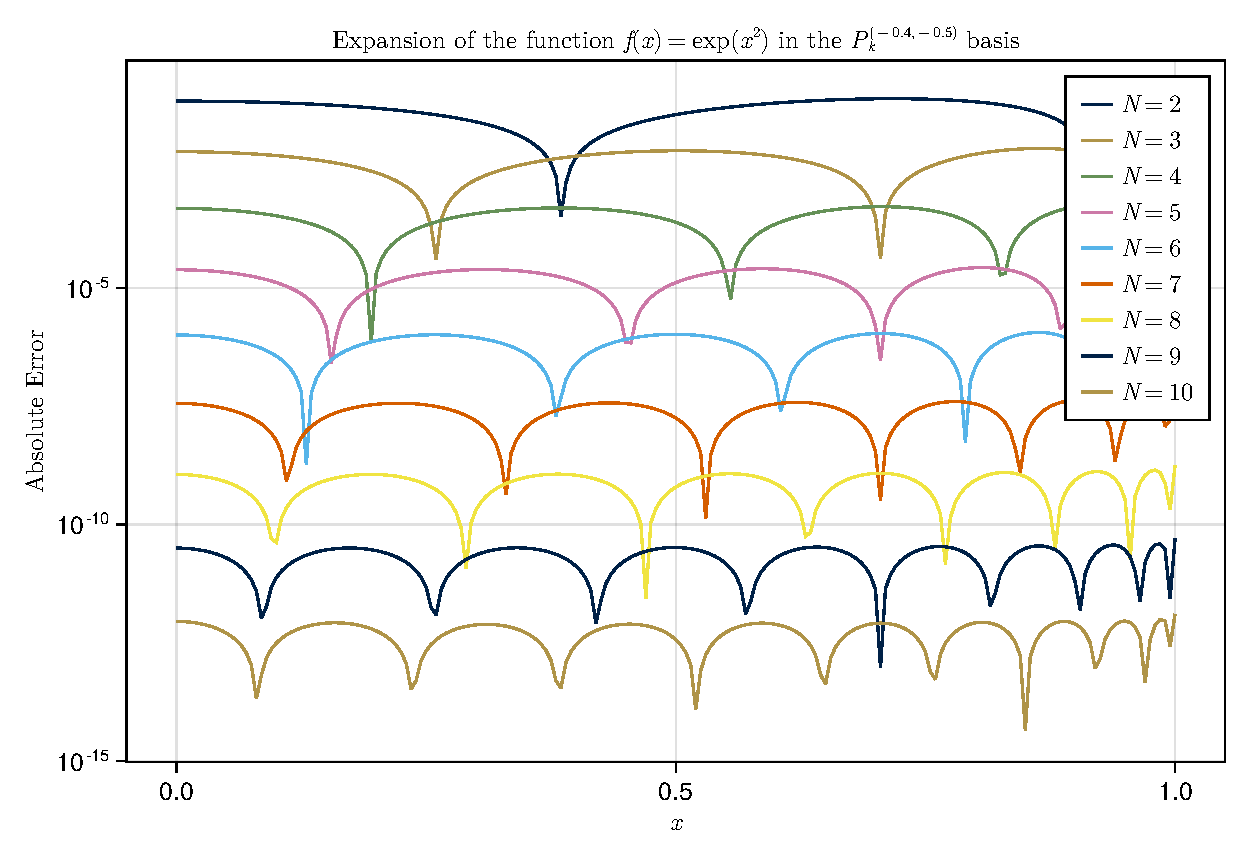
\includegraphics[width=0.7\linewidth]{results/jacobi-expansions.pdf}
  \caption[Convergence of Jacobi basis expansion]{Convergence of the Jacobi polynomial expansion $f_N(x) = \sum_{k=0}^{N-1} P_k^{(a, b)}(x)$ of an example function $f(x) = \e^{x^2}$ with $a = -\frac{3}{4}$ and $b = -\frac{1}{2}$. Each added term improves the absolute error between the function and its expansion by a factor, so we have exponential convergence. The number of ``arches'' of each solution error function, occuring from the roots of $f(x) - f_N(x)$, approximately equals the order $N$.}
\end{figure}

% TODO: Convergence speed according to theory is...?

\begin{definition}{Gegenbauer Polynomials}{gegenbauer-polynomials}
  \begin{center}\rule{0.5\linewidth}{0.5pt}\end{center}

  \hypertarget{alias-ultraspherical-polynomials}{%
    \subsection{alias: Ultraspherical
      Polynomials}\label{alias-ultraspherical-polynomials}}

  Are a special case of the Jacobi Polynomials (cf. \Cref{def:jacobi-polynomials}) and form an
  Orthonormal Basis (cf. \Cref{def:orthonormal-basis}) under the weight given by
  \[w(x)=(1+x)^\alpha\]
\end{definition}

\begin{definition}{Chebyshev Polynomials}{chebyshev-polynomials}
  Of the first kind: \[T_k(x)\] Of the second kind: \[U_k(x)\] Also have a
  {[}{[}Three-Term Recurrence Relationship{]}{]}.
\end{definition}


In order to obtain a recurrence relationship between the coefficients later, we make use of the Jacobi matrix (cf. \Cref{def:jacobi-matrix}).
\begin{remark}{}{jacobi-matrix}
  The Jacobi operator is the matrix \(X \in \R^{N \times N}\) satisfying
  $$x \cdot \vec{P}^{(a,b)}(x) = \vec{P}^{(a,b)}(x) \cdot X^T\,.$$
\end{remark}

The terms in the Jacobi operator are closely connected to the three-term recurrence relationship (cf. \Cref{thm:three-term-recurrence-relationship}), even making the matrix tridiagonal.


Finally, now that we have established the basis functions, we can write down an ansatz $\rho: B_1(\vec{0}) \mapsto \R$ for the solution of \hyperref[sec:the-problem]{the problem}, of the form
\begin{equation}
  \rho(\vec{x}) := \left(1-\norm{\vec{x}}^{2}\right)^{m - \frac{\alpha + d}{2}} \sum_{k=0}^{N-1} \rho_k P_{k}^{\left(m - \frac{\alpha + d}{2},\frac{d-2}{2}\right)}(2 \norm{\vec{x}}^{2}-1)\,.
  \label{eq:ansatz}
\end{equation}
with $P_k^{(a, b)}$ the Jacobi polynomials and $\{\rho_k\}_{k=0, ..., N-1}$ the coefficients.
% TODO: is it alpha or beta in the exponent of (1-y\^{}2)?

The spectral method can then be written as a linear system involving a matrix (operator).
\begin{definition}{Operator}{operator}
  Either the attractive or the repulsive operator can be sparse.

  Obtained using {[}{[}Theorem 2.16{]}{]}. Derivation of the exact
  row/column form on paper ( \#include in My Dissertation (cf. \Cref{def:my-dissertation}))

  \begin{itemize}
    \tightlist
    \item
          {[} {]} What does the solver look like for other kernels?
  \end{itemize}
\end{definition}

\begin{theorem}{Power Law Potential of the $n$th Jacobi Polynomial}{theorem216}
  On the $d$-dimensional unit ball $B_1(\vec{0})$ the power law potential, with power $\alpha \in(-d,2+2m-d)$, $m\in\mathbb{N}_0$ and $\beta>-d$, of the $n$th weighted radial Jacobi polynomial $(1-\norm{\vec{y}}^2)^{m-\frac{\alpha+d}{2}}P_n^{\left(m-\frac{\alpha+d}{2},\frac{d-2}{2}\right)}\left(\jacobiarg{y}\right)$ reduces to a Gaussian hypergeometric function as follows:
  \begin{align*}
    I_{m,n}^{\alpha,\beta}(\vec{x}) & = \int_{B_1(\vec{0})} \norm{\vec{x}-\vec{y}}^\beta \left(1-\norm{\vec{y}}^2\right)^{m-\frac{\alpha+d}{2}} P_{n}^{\left(m-\frac{\alpha+d}{2},\frac{d-2}{2}\right)}\left(\jacobiarg{y}\right) \dd\vec{y}                                                                                                                                                                                                             \\
                                    & = \tfrac{\pi ^{d/2} \Gamma \left(1+\frac{\beta}{2}\right) \Gamma \left(\frac{\beta+d}{2}\right) \Gamma \left(m+n-\frac{\alpha+d}{2}+1\right)}{\Gamma \left(\frac{d}{2}\right) \Gamma (n+1) \Gamma \left(\frac{\beta}{2}-n+1\right) \Gamma \left(\frac{\beta-\alpha}{2}+m+n+1\right)}{}_2F_1\left(\begin{matrix}n-\frac{\beta}{2}, -m-n+\frac{\alpha-\beta}{2} \\\frac{d}{2}\end{matrix};\norm{\vec{x}}^2\right)\,.
  \end{align*}
\end{theorem}

\begin{proof}[Proof (adapted from \cite{2021-arbitrary-dimensions}, Section 2.5)]
  ~\\
  We begin by applying \Cref{lemma:jacobi-polynomial-series} to the inside of the integrand.
  \begin{align*}
    I := \int_{B_1(\vec{0})} & \norm{\vec{x}-\vec{y}}^\beta \weight{y} \jacobi[n]{y} \dd\vec{y}                                                                                             \\
                             & = C_{a,b,n} \sum_{k=0}^n \binom{n}{k} C_{a,b,n,k} \int_{B_1(\vec{0})} \norm{\vec{x}-\vec{y}}^\beta \weight{y} \left(\norm{\vec{y}}^2 - 1\right)^k \dd\vec{y} \\
                             & = C_{a,b,n} \sum_{k=0}^n \binom{n}{k} C_{a,b,n,k} (-1)^k \int_{B_1(\vec{0})} \norm{\vec{x}-\vec{y}}^\beta \weight[a+k]{y} \dd\vec{y}
  \end{align*}
  where $a := m-\frac{\alpha+d}{2}$ and $b := \frac{d-2}{2}$.
  Note that from the first to the second line, we used $\frac{z-1}{2} = \frac{2\norm{\vec{y}}^2-1 - 1}{2} = \norm{\vec{y}}^2 - 1$.

  The constants are
  \begin{align*}
    C_{a,b,n}   & := \frac{\Gamma(a+1+n)}{n! \Gamma(1+a+b+n)}     \\
    C_{a,b,n,k} & := \frac{\Gamma(1+a+b+n + k)}{\Gamma(a+1+k)}\,.
  \end{align*}

  We identify the remaining integral as the Riesz potential $I_{\beta+d}[u](\vec{x})$, cf. \Cref{def:riesz-potential}, of the function $u(\vec{y}) := \left(1-\norm{\vec{y}}^2\right)^{a+k}$, which we can evaluate using Lemma 2.4 from \cite{2011-porous-medium-1}:
  \begin{align*}
    \int_{B_1(\vec{0})} & \norm{\vec{x}-\vec{y}}^\beta \weight[a+k]{y} \dd\vec{y} = c_{\beta+d} I_{\beta+d}\left[\vec{y} \mapsto \left(1-\norm{\vec{y}}^2\right)^{a+k}\right](\vec{x}) \\
                        & = c_{\beta+d} C_{a+k, \beta, d} \cdot {}_2F_1\left(\begin{matrix}\frac{d-(\beta+d)}{2}, -a-k-\frac{\beta+d}{2} \\d/2\end{matrix}; \norm{\vec{x}}^2\right)    \\
                        & = c_{\beta+d} C_{a+k, \beta, d} \cdot {}_2F_1\left(\begin{matrix}-\beta/2, -m-k+\frac{\alpha-\beta}{2} \\d/2\end{matrix}; \norm{\vec{x}}^2\right)\,,
  \end{align*}
  as $-a-k-\frac{\beta+d}{2} = -m + \frac{\alpha+d}{2} -k - \frac{\beta+d}{2} = -m-k+\frac{\alpha-\beta}{2}$ with constants
  \begin{align*}
    c_{\beta+d}       & := \frac{2^{\beta+d} \pi^{d/2} \Gamma\left(\frac{\beta+d}{2}\right)}{\Gamma(-\beta/2)}                      \quad \text{\textcolor{gray}{from aforementioned definition of the Riesz potential}} \\
    C_{a+k, \beta, d} & := \frac{\Gamma(a+k+1) \Gamma(-\beta/2)}{2^{\beta+d}\Gamma(d/2) \Gamma\left(a+k+\frac{\beta+d}{2}+1\right)} \quad \text{\textcolor{gray}{from Lemma 2.4}}\,,
  \end{align*}
  and therefore
  $$c_{\beta+d} C_{a+k, \beta, d} = \frac{\cancel{2^{\beta+d}} \pi^{d/2} \Gamma\left(\frac{\beta+d}{2}\right) \Gamma(a+k+1) \cancel{\Gamma(-\beta/2)}}{\cancel{\Gamma(-\beta/2)} \cancel{2^{\beta+d}}\Gamma(d/2) \Gamma\left(a+k+\frac{\beta+d}{2}+1\right)} = \frac{\pi^{d/2}B\left(\tfrac{\beta+d}{2}, a+k+1\right)}{\Gamma(d/2)}\,,$$
  using \Cref{eq:beta-gamma}.
  So that finally,
  \begin{align*}
    \int_{B_1(\vec{0})} & \norm{\vec{x}-\vec{y}}^\beta \weight[a+k]{y} \dd\vec{y}                                                                                                                                                         \\
                        & =\frac{\pi^{d/2}}{\Gamma(d/2)} B\left(\tfrac{\beta+d}{2}, m-\tfrac{\alpha+d}{2}+k+1\right) \cdot {}_2F_1\left(\begin{matrix}-\beta/2, -m-k+\frac{\alpha-\beta}{2} \\d/2\end{matrix}; \norm{\vec{x}}^2\right)\,.
  \end{align*}

  Plugging this back into the original form above, carrying along the same parameters,
  \begin{align*}
    I = C_{a,b,n} \sum_{k=0}^n \binom{n}{k} C_{a,b,n,k} (-1)^k \frac{\pi^{d/2}}{\Gamma(d/2)} B\left(\cdot, \cdot\right) {}_2F_1\left(\dots; \norm{\vec{x}}^2\right)\,
  \end{align*}
  we can apply Equation (2.1) in \cite{2021-arbitrary-dimensions} after some algebra, the special case of an identity given in \cite{1986-crazy-hypergeometric-properties} to obtain a ${}_3F_2$ (three terms in the numerator, two in the denominator) function
  \begin{align*}
    I \propto {}_3F_2\left(\begin{matrix}-\beta/2, n-\beta/2, -m-n+\frac{\alpha-\beta}{2} \\d/2, -\beta/2\end{matrix}; \norm{\vec{x}}^2\right)\,,
  \end{align*}
  which we expand into its \Cref{def:generalised-hypergeometric-series} to see that two terms cancel:
  \begin{align*}
    I \propto \sum_{k=0}^{\infty} \frac{\cancel{(-\beta/2)_k}, (n-\beta/2)_k, \left(-m-n+\frac{\alpha-\beta}{2}\right)_k}{(d/2)_k \cancel{(-\beta/2)_k}} \frac{\norm{\vec{x}}^{2k}}{k!}\,,
  \end{align*}
  which results back in a ${}_2F_1$ function (two terms in the numerator, one in the denominator), the so-called Gaussian hypergeometric function, cf. \Cref{lemma:gaussian-hypergeometric-function}, and after combining $C_{a,b,n}$, $C_{a,b,n,k}$, $\frac{\pi^{d/2}}{\Gamma(d/2)}$ with the gamma-function expansion of $B\left(\tfrac{\beta+d}{2}, m-\tfrac{\alpha+d}{2}+k+1\right)$ according to \Cref{eq:beta-gamma}, and cancelling terms, one finally obtains
  $$I = \tfrac{\pi^{d/2} \Gamma \left(1+\frac{\beta}{2}\right) \Gamma \left(\frac{\beta+d}{2}\right) \Gamma \left(m+n-\frac{\alpha+d}{2}+1\right)}{\Gamma \left(\frac{d}{2}\right) \Gamma (n+1) \Gamma \left(\frac{\beta}{2}-n+1\right) \Gamma \left(\frac{\beta-\alpha}{2}+m+n+1\right)}{}_2F_1\left(\begin{matrix}n-\frac{\beta}{2}, -m-n+\frac{\alpha-\beta}{2} \\\frac{d}{2}\end{matrix};\norm{\vec{x}}^2\right)\,,$$
  concluding the proof.
\end{proof}

Lemma 2.4 from \cite{2011-porous-medium-1,1967-formulas-and-theorems} is based on the \textit{Weber-Schafheitlin} integral of two Bessel functions given in \cite{1945-bessel-integral}.
The Weber-Schafheitlin integrals are related to the fractional Laplacians of aforementioned functions because the Fourier transform of ${}_2F_1$ is a Bessel function.
For a more generalised version of Lemma 2.4, see \cite{2014-barenblatt}.

Also note that for even integer $\beta$, the prefactor in \Cref{thm:theorem216} sometimes contains an expression of the form $\Gamma(-n),\, n \in \N$ which in principle leads to undefined behaviour (cf. \Cref{def:gamma-function} together with the property that $k \Gamma(k) = \Gamma(k+1)$).
However, one can consider the limit as $x \in \R^+$ approaches an integer $n$ to find that
$$\lim_{x \goesto n} \Gamma(-x) = (-1)^{n-1} \infty\,, \quad\text{or equivalently}\quad \lim_{x \goesto n} \frac{1}{\Gamma(-x)} = 0\,,$$
in which case we are lucky because $\Gamma(\beta/2-n+1)$ appears in the denominator of the prefactor and without any singularities in the numerator we can safely evaluate the entire expression to $0$.

Because $I_{m,n}^{\alpha,\beta}(\vec{x})$ only depends on the squared radius $r^2 = \norm{\vec{x}}^2$, let it also be denoted by $I_{m,n}^{\alpha,\beta}(r^2) = I_{m,n}^{\alpha,\beta}(\vec{x})$.
Further, let
\begin{equation}
  \bar{I}_{m,n}^{\alpha,\beta} := \frac{\left\langle x \mapsto I\left(\frac{x+1}{2}\right), P_0^{(a, b)} \right\rangle}{\left\langle P_0^{(a, b)}, P_0^{(a, b)} \right\rangle} = \frac{1}{h_0^{(a, b)}} \int_{-1}^{1} I_{m,n}^{\alpha,\beta}\left(\frac{x+1}{2}\right) w^{(a,b)}(x) \,\ddx\,,
  \label{eq:0th-coeff-of-I}
\end{equation}
denote the 0th coefficient in a Jacobi expansion of $I_{m,n}^{\alpha,\beta}(\vec{x})$ (recall that $r^2 = \frac{x+1}{2}$ and $P_0^{(a, b)}(x) = 1$) with $h_k := \left\langle P_k^{(a, b)}, P_k^{(a, b)} \right\rangle$ the normalisation coefficients of the basis.


\begin{lemma}{Mass of the Solution}{mass}
  For a given solution $\rho: B_1(\vec{0}) \mapsto \R$, its \textit{mass} $M \in \R$ is given by \Cref{eq:measure-mass}.
  Provided the appropriate ansatz given in \Cref{eq:ansatz}, an expansion of weighted radial Jacobi polynomials with coefficients $\rho_k$, its \textit{mass} is given by
  \begin{align*}
    M := \int_{\supp(\rho)} \rho(y) \,\ddy = \frac{\pi^{{d/2}}\Gamma (a+1)}{\Gamma \left(a+{d/2}+1\right)}\, \rho_0\,,
  \end{align*}
  so solely depending on the first coefficient $\rho_0$.
\end{lemma}
\begin{proof}[Proof (adapted from \cite{2021-arbitrary-dimensions})]
  To shorten notation, let $b := \frac{d-2}{2}$.
  The domain and radial symmetry of our problem suggests the use of hyperspherical coordinates:
  \begin{align*}
    M = \int_{B_1(\vec{0})} \rho(\vec{x}) \,\dd\vec{x} & = \sum_{k=0}^{N-1} \rho_k \int_{B_1(\vec{0})} \weight{x} P_k^{(a,b)}(\jacobiarg{x}) \,\dd\vec{x}                          \\
                                                       & =\sum_{k=0}^{N-1} \rho_k \int_{\partial B_1(\vec{0})} \dd\Omega \int_{r=0}^1 (1-r^2)^a P_k^{(a,b)}(2r^2-1) r^{d-1} \,\ddr \\
                                                       & = \Omega_d \sum_{k=0}^{N-1} \rho_k \int_{r=0}^1 (1-r^2)^a P_k^{(a,b)}(2r^2-1) r^{d-1} \,\ddr\,,
  \end{align*}
  where $\Omega_d = {2\pi^{d/2}} / {\Gamma({d/2})}$ is the surface area of the $d$-dimensional hypersphere (cf. \Cref{lemma:surface-area}) with radius $R = 1$.
  % Note that working with a finite expansion ($N < \infty$), we automatically have
  % $$\int_{B_1} \sum_{k=0}^{N-1} |\rho_k (1-|y|^2)^a P_k^{(a,b)}(2|y|^2-1)| \,\ddy < \infty\,,$$
  % so the exchange of integration and infinite sum in the first line is justified by the Fubini-Tonelli theorem.
  Substituting $u := 2r^2-1$, therefore $r^2 = \frac{1+u}{2}$ and $(1-r^2)^a = \left(\frac{1-u}{2}\right)^a = 2^{-a} (1-u)^a$ as well as $\ddr = \frac{\ddu}{4r}$,
  \begin{align*}
    M & = 2^{-a} \Omega_d \sum_{k=0}^{N-1} \rho_k \int_{u=-1}^1 (1-u)^a P_k^{(a,b)}(u) r^{d-1} \,\frac{\ddu}{4r} \\
      & = 2^{-2} 2^{-a} \Omega_d \sum_{k=0}^{N-1} \rho_k \int_{-1}^1 (1-u)^a P_k^{(a,b)}(u) r^{d-2}\,\ddu\,,
  \end{align*}
  we notice that $r^{d-2} = \left(\frac{1+u}{2}\right)^{\frac{d-2}{2}} = 2^{-b} (1+u)^b$ and so we have
  \begin{align*}
    M & = 2^{-2} 2^{-a} 2^{-b} \Omega_d \sum_{k=0}^{N-1} \rho_k \int_{-1}^1 (1-u)^a (1+u)^{b} P_k^{(a,b)}(u) \,\ddu                                                 \\
      & = 2^{-(2+a+b)} \Omega_d \sum_{k=0}^{N-1} \rho_k \int_{-1}^1 (1-u)^a (1+u)^{b} P_k^{(a,b)}(u) P_0^{(a, b)}(u) \,\ddu                                         \\
      & = 2^{1-(2+a+b)} \frac{\pi^{d/2}}{\Gamma(d/2)} \sum_{k=0}^{N-1} \rho_k \, \frac{2^{a+b+1} \Gamma (a+1) \Gamma (b+1)}{0! (a+b+1) \Gamma (a+b+1)} \delta_{0,k} \\
      & = \frac{\pi^{{d/2}}\Gamma (a+1)}{\Gamma \left(a+{d/2}+1\right)} \,\rho_0\,,
  \end{align*}
  which relies on the classical orthogonality condition of the Jacobi polynomials given in \Cref{thm:jacobi-orthogonality-condition} with the $0$th polynomial $P_0(u) = 1$.
\end{proof}

\begin{lemma}{Surface area of the hypersphere}{surface-area}
  The surface area of the d-dimensional hypersphere $\partial B_R(\vec{0})$ is given by
  $$\Omega_{d}(R) = \frac{\dd}{\dd R} V_d(R) = \frac{\dd}{\dd R} \left(\frac{2 \pi^{d/2}}{d \Gamma(d/2)} R^d\right) = \frac{2\pi^{d/2}}{\Gamma({d/2})} R^{d-1}\,.$$
\end{lemma}
\begin{proof}
  We find $\Omega_d$ by evaluation of the $d$-dimensional Gaussian integral
  $$I_d := \int_{\R^d} \e^{-\norm{\vec{x}}^2}\,\dd\vec{x} = \int_{\R} \ddx_1 ... \int_{\R} \ddx_d\, \e^{-x_1^2-...-x_d^2} = \left(\int_{\R} \e^{-x_1^2} \,\ddx_1\right)^d = (I_1)^d\,,$$
  using Fubini's theorem ($I_d < \infty$).
  Considering the case $d = 2$, we have
  $$I_2 = \int_{\R^2} \e^{-\norm{\vec{x}}^2} \,\dd\vec{x} = \int_0^{2\pi} \dd\theta \int_0^\infty r \e^{-r^2} \,\ddr = -2\pi \int_{0}^{-\infty} \e^u \,\frac{\ddu}{2} = \pi \int_{-\infty}^0 \e^u \,\ddu = \pi\,,$$
  taking the classical approach of transitioning to polar coordinates $r, \theta$ (with Jacobi determinant $r^{d-1}$ in the $d$-dimensional case) immediately leading us to $I_1 = \sqrt{\pi}$. Generalising this to higher dimensions $d$ with hyperspherical coordinates,
  $$I_d = \int_{\R^d} \e^{-\norm{\vec{x}}^2} \,\dd\vec{x} = \Omega_d \int_0^\infty r^{d-1} \e^{-r^2}\,\ddr = \Omega_d \int_0^\infty s^{{d/2}-1} \e^{-s} \frac{\dds}{2} = \frac{\Omega_d}{2} \Gamma(d/2)\,,$$
  where once again $r := \norm{\vec{x}}$ and using a substitution $s := r^2$, we must find equality with the above result $I_d = \pi^{d/2}$,
  $$I_d = \pi^{d/2} \overset{!}{=} \frac{1}{2}\Omega_d \Gamma(d/2) \qLRq \Omega_d = \frac{2\pi^{d/2}}{\Gamma(d/2)}\,.$$
  Now integrating over the $R$-ball $B_R(\vec{0})$, we obtain $V_d(R) := |B_R(\vec{0})| = \Omega_d \int_0^R r^{d-1} \,\ddr = \frac{\R^d \Omega_d}{d}$ and therefore $\Omega_{d}(R) = \frac{\dd V_d(R)}{\dd R} = \frac{2 \pi^{d/2}}{\Gamma(d/2)}R^{d-1}$.
\end{proof}


\section{Derivation of Operator}
Based on the {[}{[}Three-Term Recurrence Relationship{]}{]}.

One can even determine an explicit relationship between the coefficients
in the Jacobi expansion by considering the {[}{[}Jacobi Matrix{]}{]}.

Considering the operator $\hat{Q}^\beta[\rho]$ as in \Cref{thm:theorem216}, from the [[Ansatz]] $\rho(x)$ we have
$$\hat{Q}^{\beta}(x) = \sum_{k=1}^{N} \rho_{k} \int \norm{x-y}^{\beta}(1-\norm{y}^2)^{a}P_{k}^{(a, b)}(2\norm{y}^{2}- 1) \,\ddy$$


\begin{figure}[H]
  \centering
  \label{fig:attractive-repulsive}
  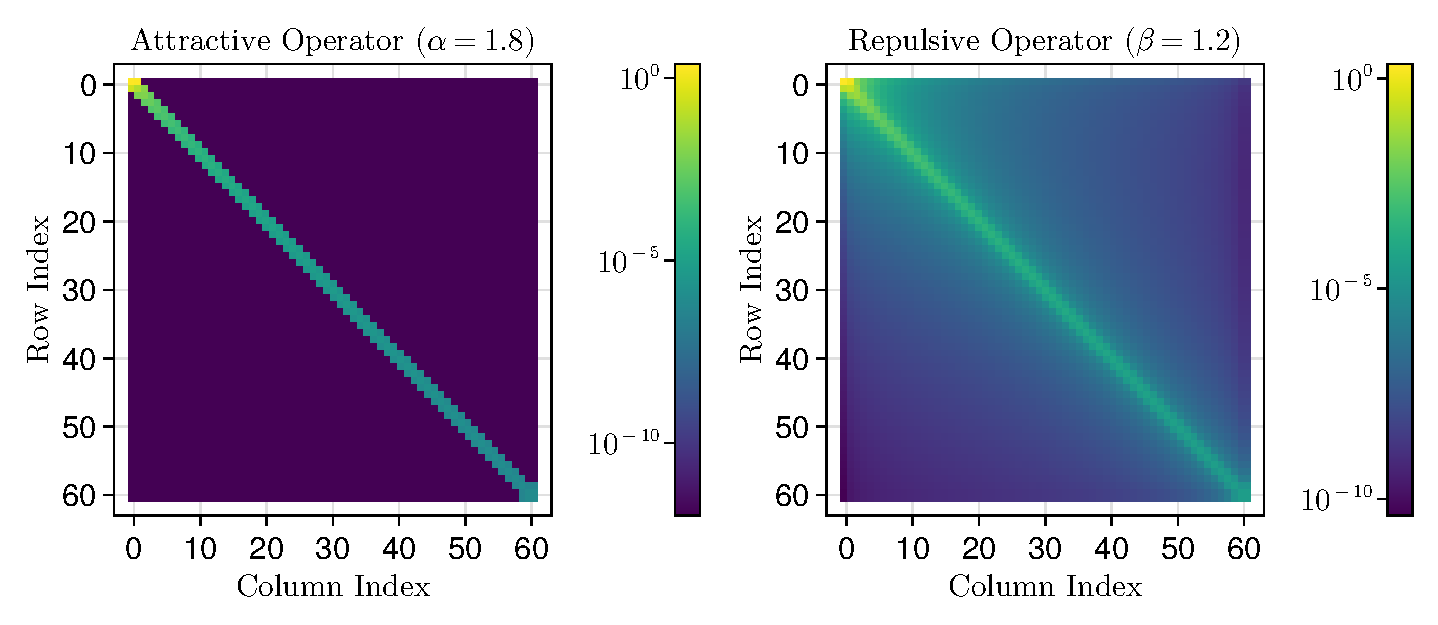
\includegraphics[width=\linewidth]{results/attrep/attractive-repulsive-operators.pdf}
  \caption[Attractive and repulsive operators.]{The attractive and repulsive operators (matrices) as given in \Cref{def:operator}, the matrix values are shown in a $\log_{10}$ color scale. Due to the choice of basis, the attractive operator is exactly banded. The repulsive parameter is only approximately banded, which the spy plots effectively demonstrate.}
\end{figure}

The bandedness of the attractive operator is due to the three-term recurrence relationship of the Jacobi polynomial basis.
% TODO.. explain

For the attractive-repulsive interaction potential, the full operator is given by
\begin{equation}
  Q_{\alpha, \beta} := \frac{R^\alpha}{\alpha} Q^\alpha - \frac{R^\beta}{\beta} Q^\beta
  \label{eq:full-attrep-operator}
\end{equation}
for some interval radius $R \in \R^+$, usually chosen as the smallest possible $R$ such that $\supp(\rho) \subseteq [-R, R]$.

\begin{figure}[H]
  \centering
  \label{fig:attrep-operator}
  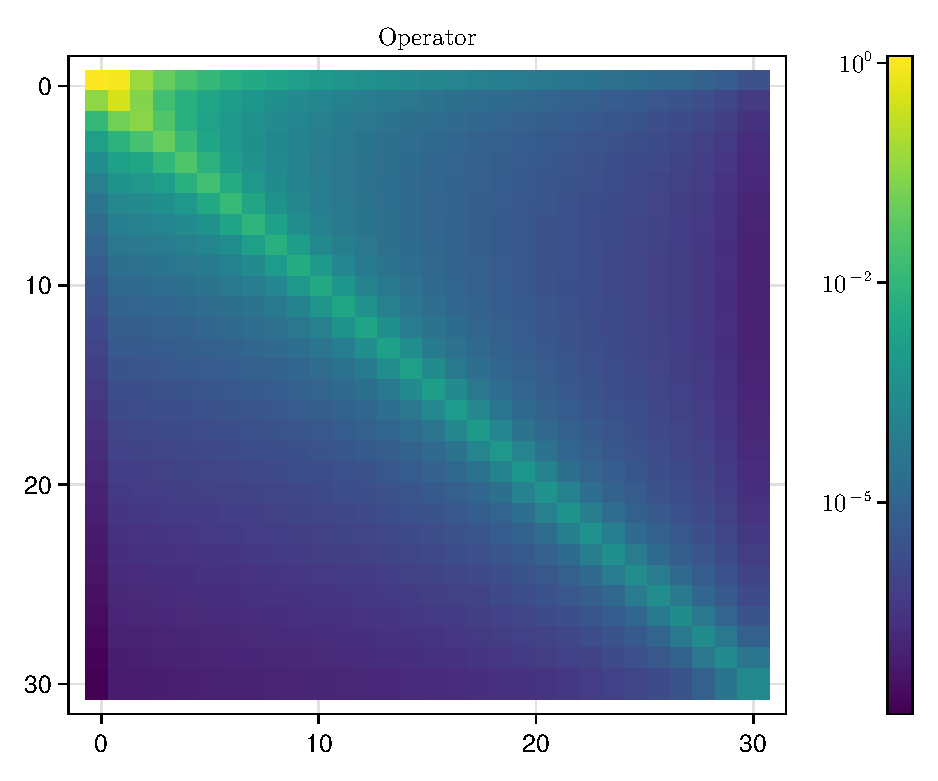
\includegraphics[width=0.5\linewidth]{results/attrep/full-operator.pdf}
  \caption[Combination of the attractive-repulsive operators]{Spy plot of $Q_{\alpha, \beta}$, the combination of the attractive-repulsive operators. Inverting this operator and applying it to $(1, 0, ..., 0)^T \in \R^N$ will yield the unnormalised coefficients $\rho_k$ of the solution expansion given in \Cref{eq:ansatz}.}
\end{figure}

\section{Results}
\begin{figure}[H]
  \centering
  \label{fig:solution-increasing-order}
  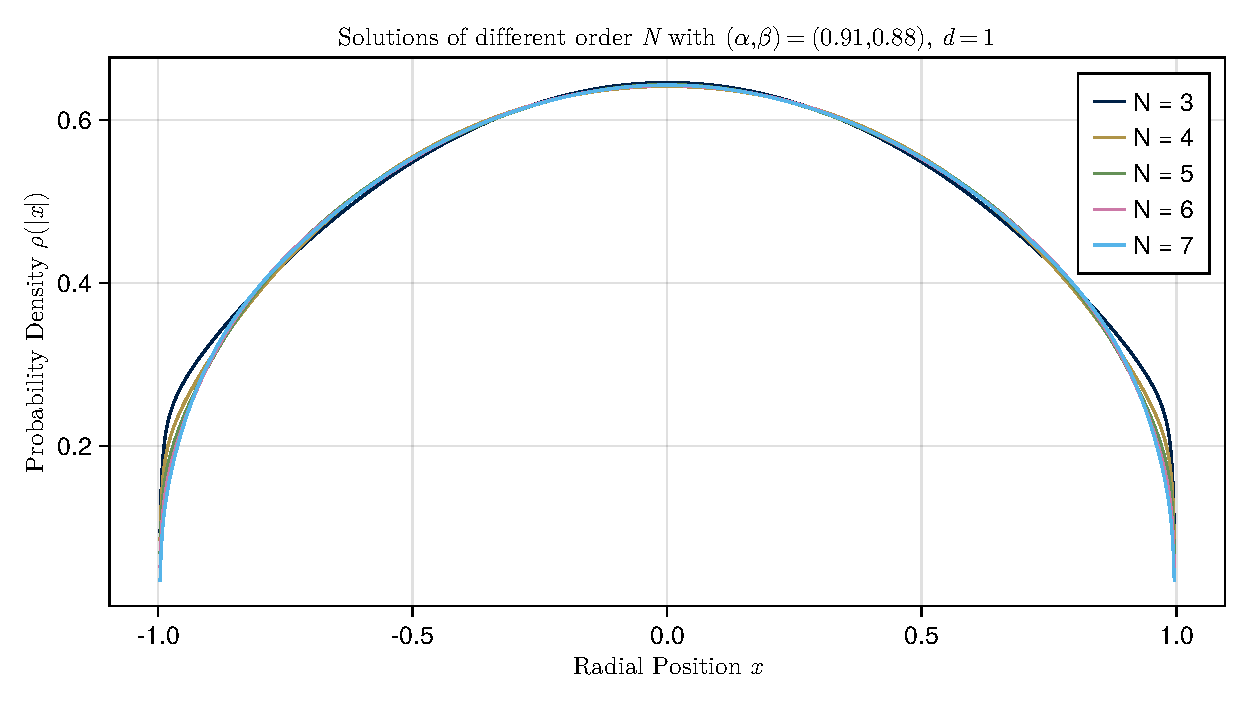
\includegraphics[width=0.8\linewidth]{results/attrep/solution-increasing-order.pdf}
  \caption[Solutions of increasing orders]{Particle density distribution function solutions $\rho$ of increasing order $N$ to the attractive-repulsive problem with interaction potential $K_{alpha, \beta}(r)$, $\alpha = 2.5$ and $\beta = 1.2$. Reflected along the y-axis for better visibility of the domain.}
\end{figure}

\section{Outer Optimisation Routine}
\begin{figure}[H]
  \centering
  \label{fig:outer-optimisation}
  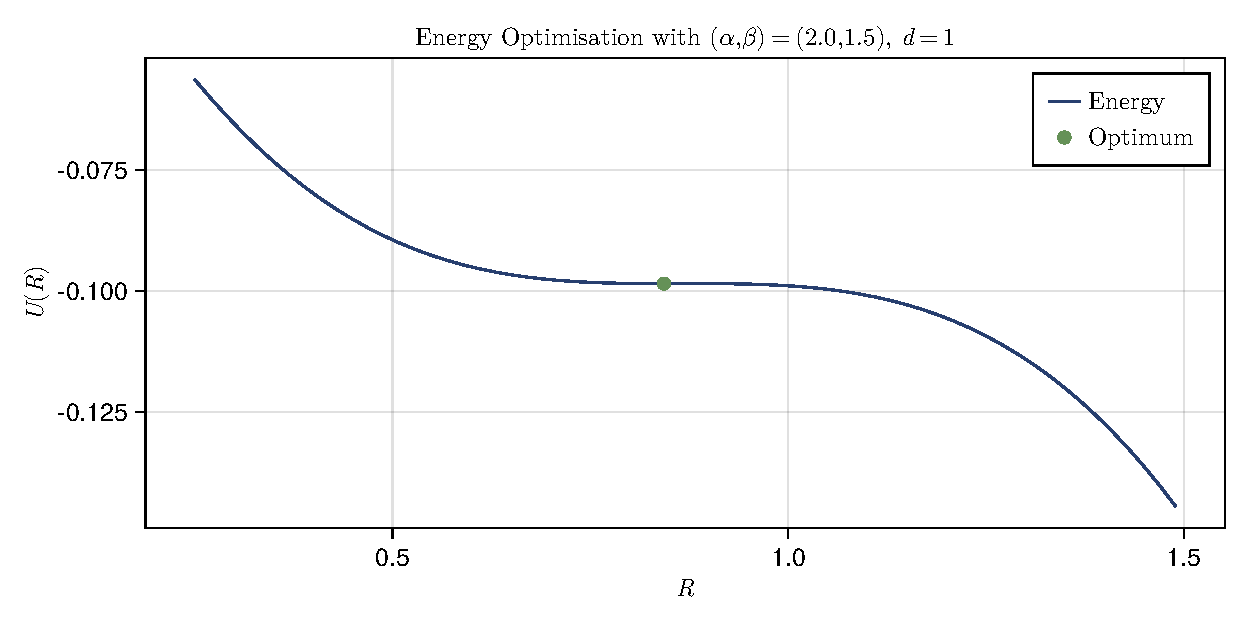
\includegraphics[width=0.8\linewidth]{results/known-analytic/outer-optimisation.pdf}
  \caption[Outer Optimisation Routine]{The total potential $U$ as a function of the support radius $R$. This is the goal function minimised by the outer optimisation routine.}
\end{figure}

Note that using this setup, the operators themselves do not need to be recomputed upon a change in $R$ (cf. \Cref{eq:full-attrep-operator}).
The provided implementation uses \gls{lru} caching to automatically store operators for a given parameter set and order $N$.

\section{Comparison with Analytic Solutions}
As introduced in \Cref{sec:analytical-solutions}, there are some analytical solutions available which allow us to perform some further analysis of the numerical method in these special cases.

\begin{figure}[H]
  \centering
  \label{fig:analytic-solution}
  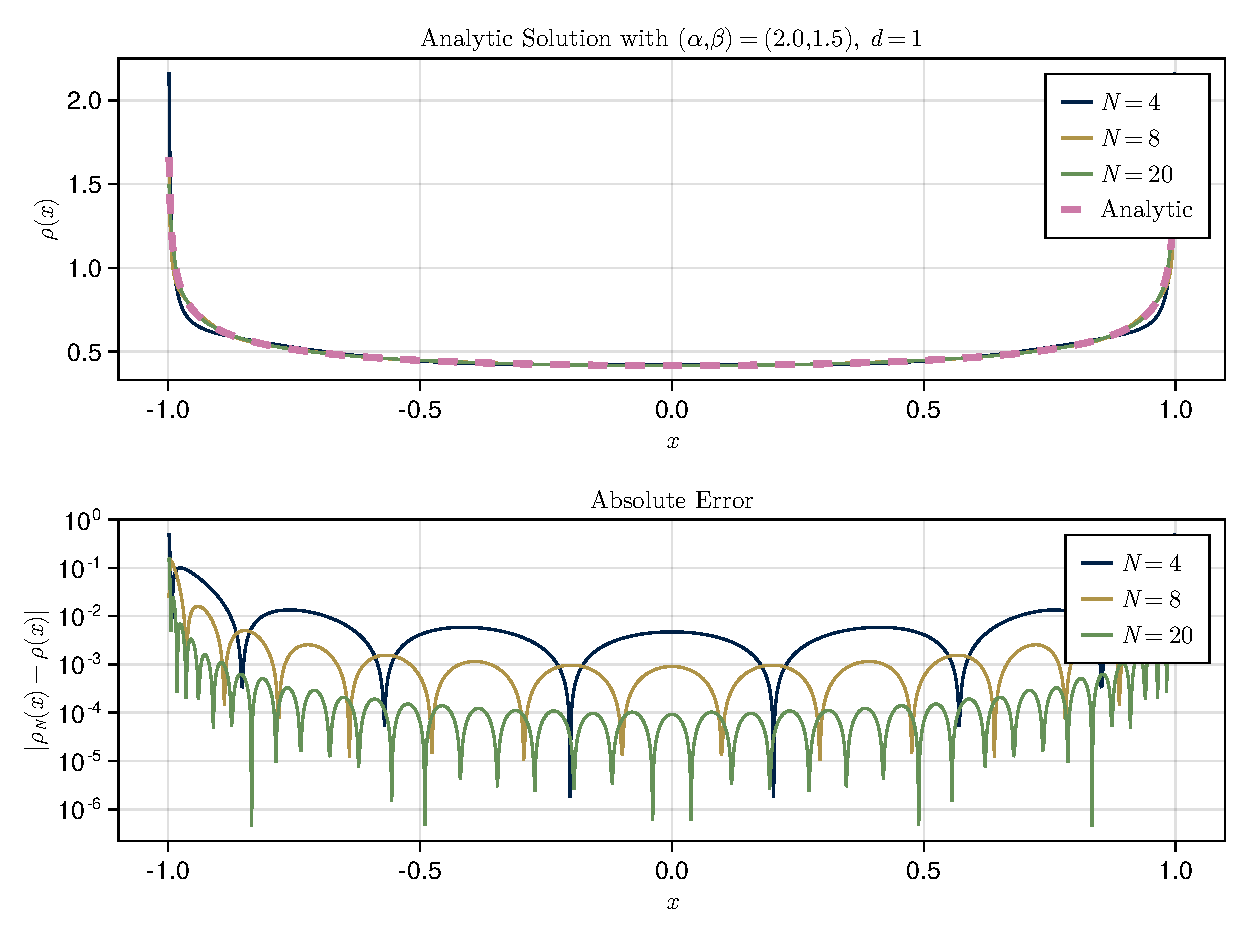
\includegraphics[width=\linewidth]{results/known-analytic/analytic-solution.pdf}
  \caption[Comparison with analytical solutions and error]{
    The analytic solution $\rho(x)$ given in \Cref{eq:analytical-solution-alpha-equal-2} compared to the (spectral method) solutions of different order $N$.
    The ``arches'' occur as a result of the roots of $\rho(x) - \rho_N(x)$, their number approximately equals the order $N$ (a polynomial of degree $N$ has $N$ roots).
  }
\end{figure}

\begin{definition}{Spectral Convergence}{spectral-convergence}
  An \(N\)-point approximation \(\varphi_N\) of a function f converges to \(f\) at spectral speed if \(|\varphi_N -f|\) decays pointwise in \([-1, 1]\) faster than \(\mathcal{O}(N^{-p})\) for any \(p = 1, 2, . . .\) so \(p \in \mathbb{N}\).
\end{definition}


\begin{figure}[H]
  \centering
  \label{fig:convergence-to-analytic}
  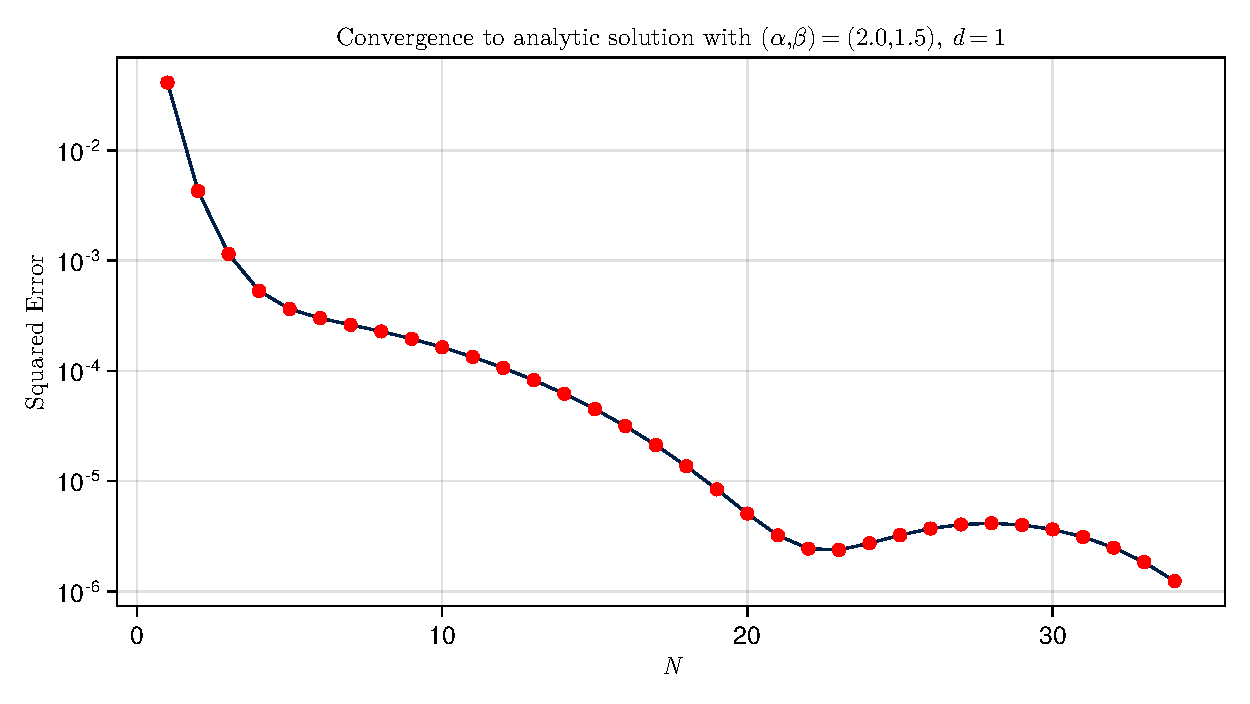
\includegraphics[width=0.8\linewidth]{results/known-analytic/convergence-to-analytic.pdf}
  \caption[Convergence to analytic solution]{Convergence of the numerical solution to the known analytic solution (cf. \Cref{eq:analytical-solution-alpha-equal-2}) in a special case where it is known, squared error plotted as a function of the highest order in the expansion $N$.}
\end{figure}

\section{Discussion}
\begin{figure}[H]
  \centering
  \label{fig:convergence}
  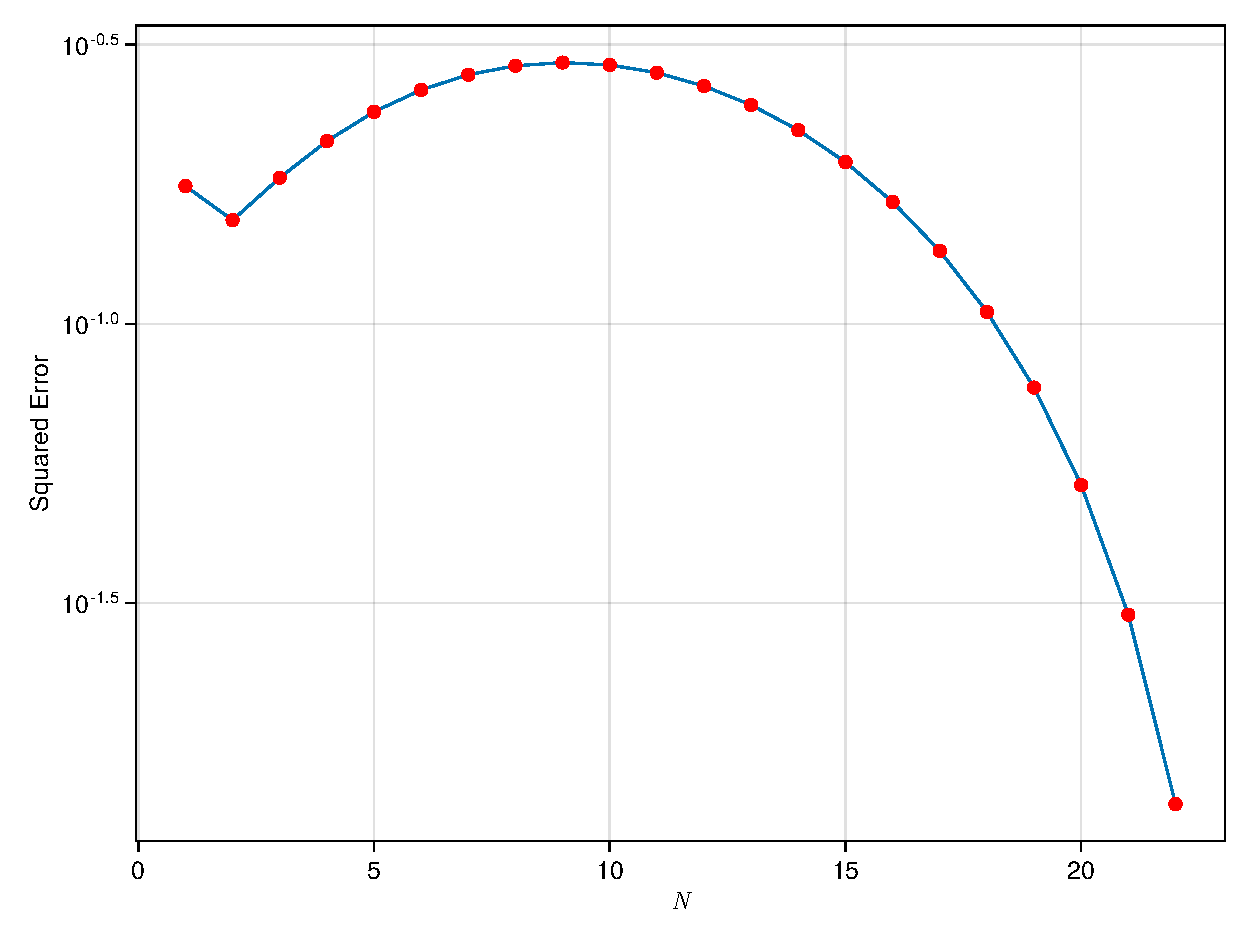
\includegraphics[width=0.8\linewidth]{results/attrep/convergence.pdf}
  \caption[Step-by-step convergence of solutions compared to order 24]{Step-by-step convergence of numerical solutions $\rho_N(x)$ as compared to $\rho_{24}(x)$, visualised using the squared error of the pointwise evaluation of both functions in $200$ points.}
\end{figure}

\begin{figure}[H]
  \centering
  \label{fig:spatial-energy-dependence}
  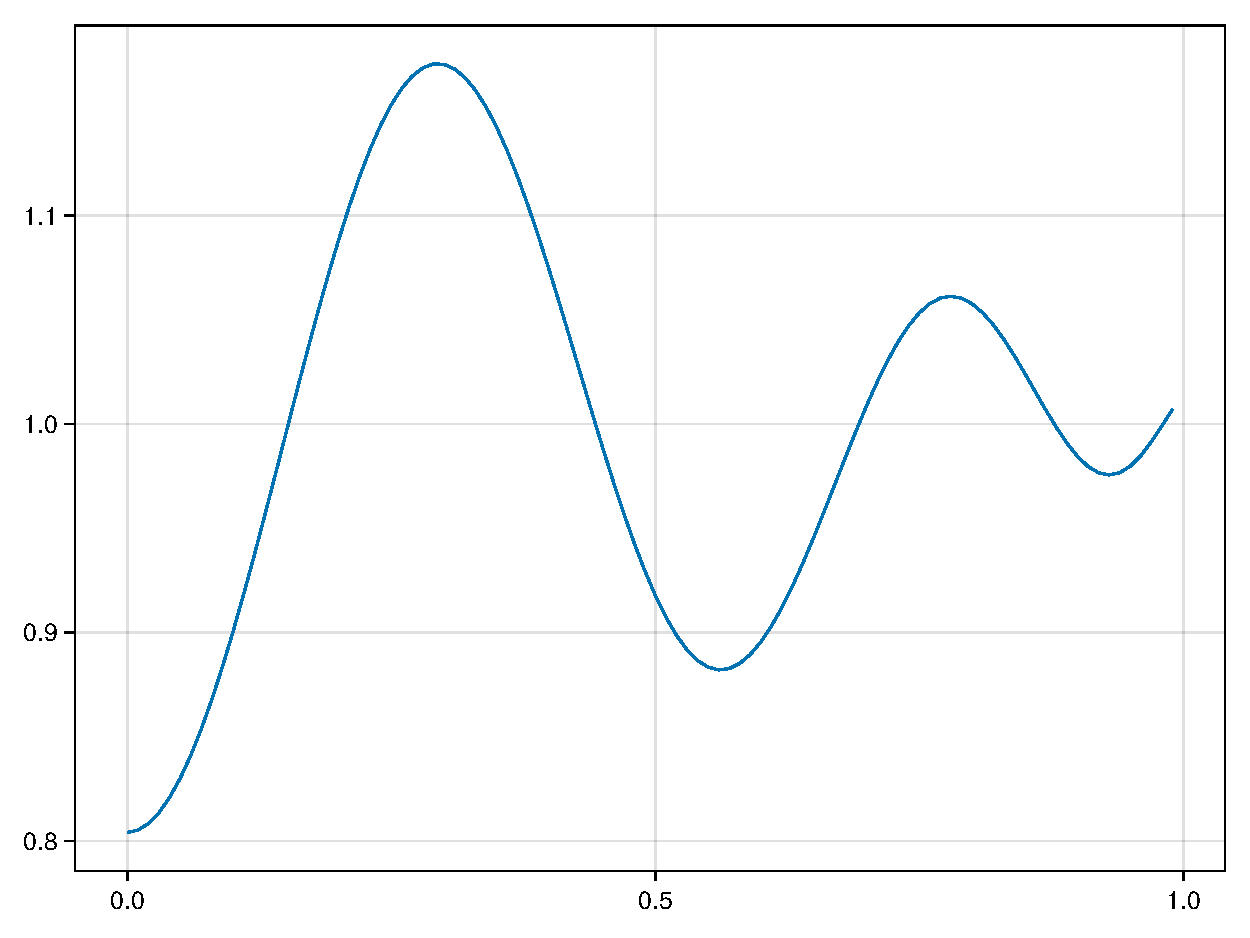
\includegraphics[width=0.7\linewidth]{results/attrep/energy-dependence-on-r.pdf}
  \caption[Spatial energy dependence on $r$]{Plot of the spatial energy dependence on $r$, for different values of the domain support radius $R$. As one can see, they are constant and this figure is only present as visual proof to increase our confidence in the construction of the spectral method.}
\end{figure}

\begin{figure}[H]
  \centering
  \label{fig:varying-parameters}
  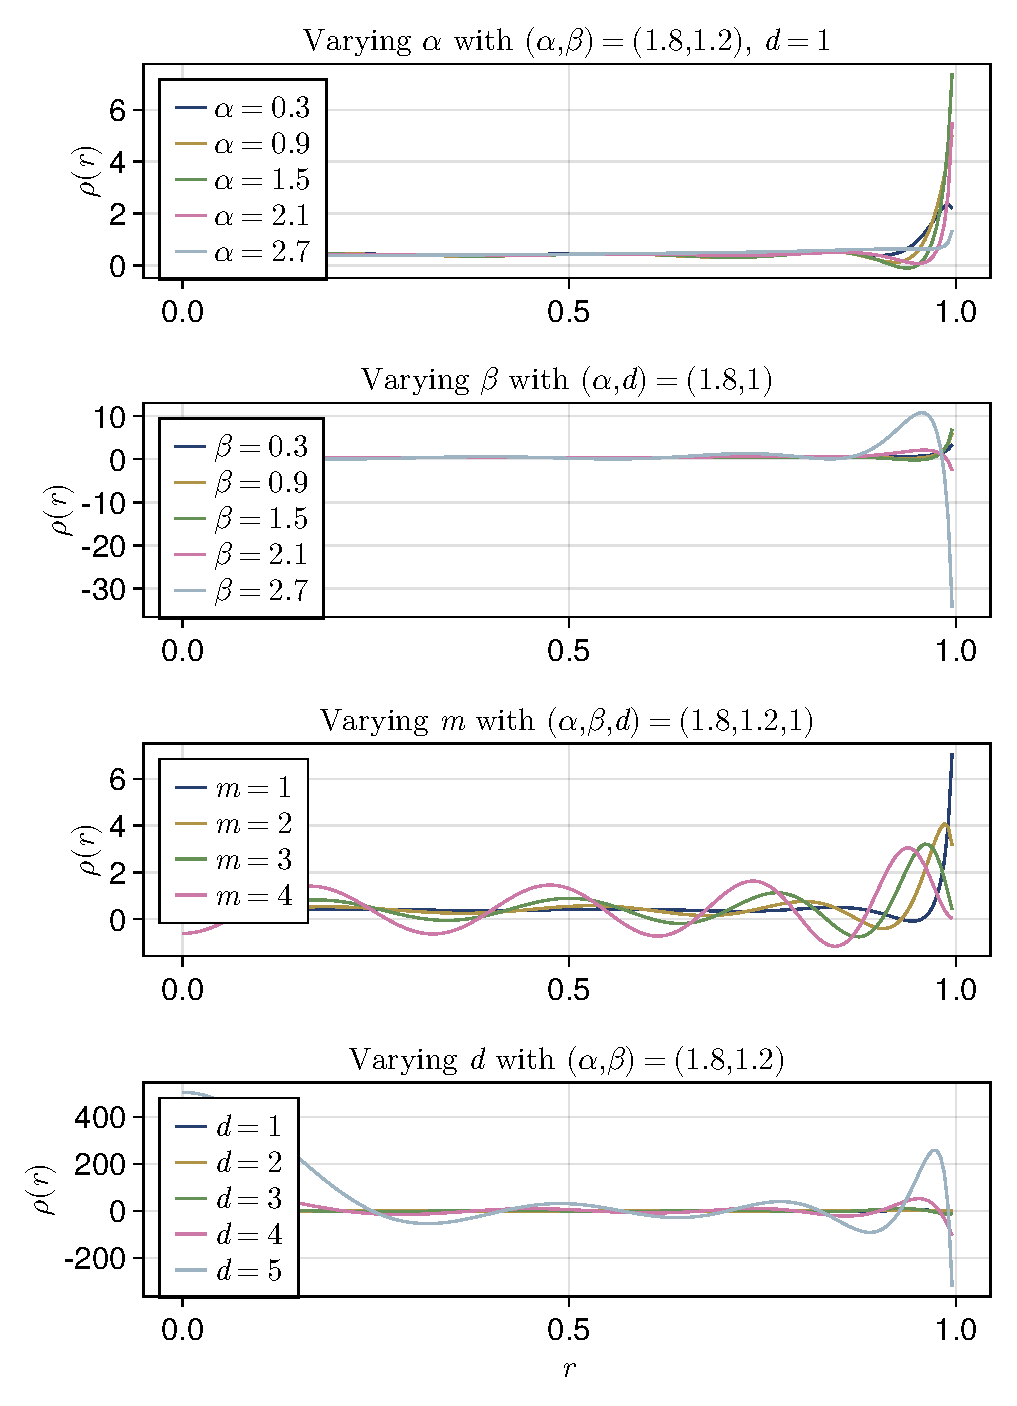
\includegraphics[width=0.9\linewidth]{results/attrep/varying-parameters.pdf}
  \caption[Varying parameters in the solver]{
    Varying different parameters in the solver to demonstrate their effect.
    See also, \Cref{fig:varying-R-solutions}.
  }
\end{figure}
